% ============================================================
% BTH04 - Yeu cau 1: Bao cao ca nhan tren Overleaf (mau Springer LNCS)
% Cach dung: Overleaf -> New Project -> Templates -> "Springer Lecture Notes in
%   Computer Science" -> Open as Template; xoa samplepaper.tex, tai len main.tex,
%   references.bib va thu muc figures/. Compiler: pdfLaTeX.
% ============================================================
\documentclass[runningheads]{llncs}

% --- Go tieng Viet (pdfLaTeX hoac XeLaTeX/LuaLaTeX) ---
\usepackage{iftex}
\ifPDFTeX
  \usepackage[T5]{fontenc}
  \usepackage[utf8]{inputenc}
\else
  \usepackage{fontspec}
  \setmainfont{TeX Gyre Termes}
\fi
\usepackage[vietnamese]{babel}

\usepackage{graphicx}
\graphicspath{{figures/}}
\usepackage[caption=false]{subfig}   % cum hinh con
\usepackage{tabularx}                % bang tu co gian do rong cot
\usepackage{booktabs}
\usepackage{amsmath,amssymb}
\usepackage[unicode]{hyperref}
\usepackage{color}
\renewcommand\UrlFont{\color{blue}\rmfamily}

\begin{document}

\title{Dự đoán kết quả học tập của học sinh bằng cây quyết định và gom nhóm K-Means}
\titlerunning{Dự đoán kết quả học tập bằng học máy}

\author{Phạm Lê Trường Thịnh\inst{1}\orcidID{0009-0002-5606-6810}}
\authorrunning{Phạm Lê Trường Thịnh}
\institute{Trường Công nghệ Thông tin và Truyền thông, Đại học Cần Thơ,
Khu II, đường 3/2, Ninh Kiều, Cần Thơ, Việt Nam\\
\email{email@student.ctu.edu.vn}}

\maketitle

\begin{abstract}
Phát hiện sớm học sinh có nguy cơ không đạt là bài toán quan trọng của khai phá dữ liệu
giáo dục. Bài báo áp dụng ba kỹ thuật học máy trên bộ dữ liệu công khai UCI Student
Performance gồm 649 học sinh: cây quyết định để phân loại Đạt/Chưa đạt, K-Means để phân
nhóm người học theo hành vi, và hồi quy tuyến tính để dự đoán điểm cuối kỳ. Cây quyết định
độ sâu 3 đạt độ chính xác 88,2\% và cho thấy điểm giữa kỳ là yếu tố quyết định; K-Means tìm
ra một nhóm rủi ro chỉ có 45\% học sinh đạt; mô hình hồi quy giải thích 88,3\% phương sai
của điểm cuối kỳ. Kết quả gợi ý có thể cảnh báo sớm ngay sau kỳ kiểm tra đầu tiên.
\keywords{Khai phá dữ liệu giáo dục \and Cây quyết định \and K-Means \and Hồi quy tuyến tính.}
\end{abstract}

% ------------------------------------------------------------
\section{Giới thiệu}\label{sec:intro}
Khai phá dữ liệu giáo dục (Educational Data Mining) dùng các kỹ thuật học máy để hiểu và
cải thiện quá trình học tập~\cite{romero2020}. Một trong những ứng dụng phổ biến nhất là dự
đoán kết quả học tập, giúp giáo viên phát hiện sớm học sinh cần hỗ trợ~\cite{shahiri2015,hellas2018}.
Các tổng quan gần đây cho thấy cây quyết định, mạng nơ-ron và các phương pháp tổ hợp như
Random Forest~\cite{breiman2001} được dùng nhiều nhất~\cite{albreiki2021}.

Bài báo này có ba đóng góp: (i) xây dựng cây quyết định dễ diễn giải để phân loại học sinh
Đạt/Chưa đạt; (ii) phân nhóm người học theo hành vi bằng K-Means; (iii) đánh giá khả năng dự
đoán điểm cuối kỳ bằng hồi quy tuyến tính. Phần~\ref{sec:data} mô tả dữ liệu,
Phần~\ref{sec:method} trình bày phương pháp, Phần~\ref{sec:result} thảo luận kết quả và
Phần~\ref{sec:conclusion} kết luận.

% ------------------------------------------------------------
\section{Dữ liệu}\label{sec:data}
\subsection{Nguồn và giấy phép}
Nghiên cứu dùng bộ dữ liệu \emph{Student Performance}~\cite{cortez2008data} của kho UCI,
giấy phép CC BY 4.0. Tệp \texttt{student-por.csv} gồm 649 học sinh trung học môn tiếng Bồ
Đào Nha với 33 thuộc tính về nhân khẩu học, gia đình, thói quen học tập và ba cột điểm
$G_1, G_2, G_3$ trên thang 0--20. Dữ liệu đã được ẩn danh từ nguồn, không chứa thông tin
định danh cá nhân.

\subsection{Tiền xử lý và khám phá}
Dữ liệu được làm sạch bằng pandas~\cite{mckinney2010} và NumPy~\cite{harris2020}: ép kiểu số cho
cột điểm, loại bản ghi trùng, mã hóa các biến nhị phân (\emph{yes/no}) thành 0/1. Nhãn phân
loại được định nghĩa là \emph{Đạt} khi $G_3 \ge 10$. Tỷ lệ đạt là 84,6\%, điểm $G_3$ trung
bình 11,91 (độ lệch chuẩn 3,23). Hình~\ref{fig:eda} tóm tắt bốn góc nhìn khám phá dữ liệu,
được vẽ bằng Matplotlib~\cite{hunter2007} và seaborn~\cite{waskom2021}.

\begin{figure}[t]
\centering
\subfloat[Phân phối điểm $G_3$\label{fig:eda-hist}]{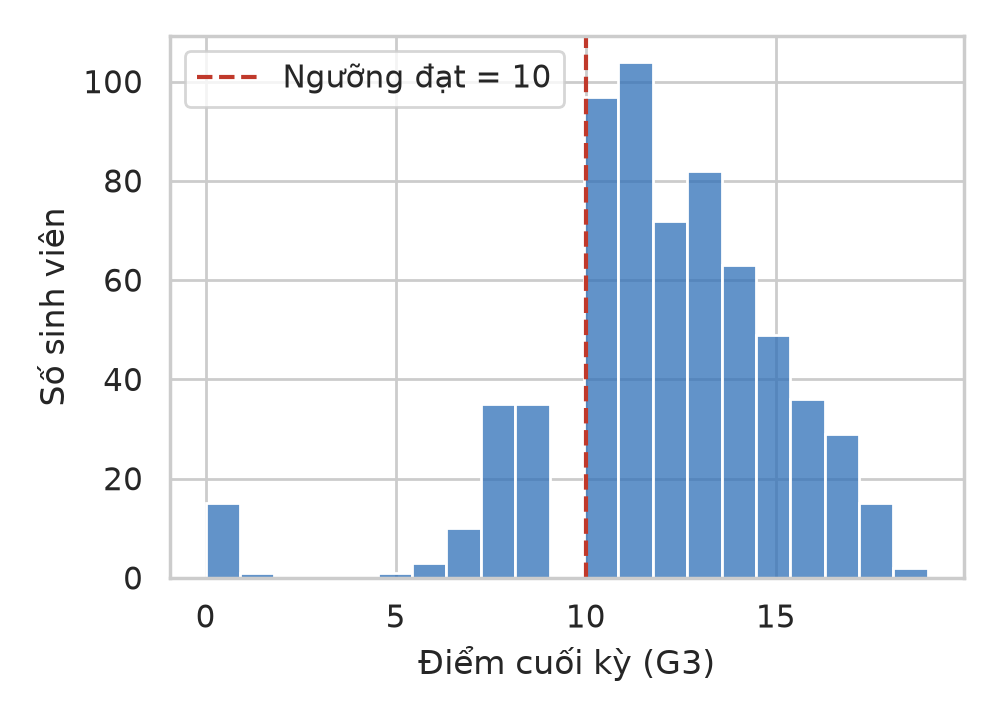
\includegraphics[width=0.48\linewidth]{eda_g3_hist}}\hfill
\subfloat[Tỷ lệ đạt theo thời gian tự học\label{fig:eda-study}]{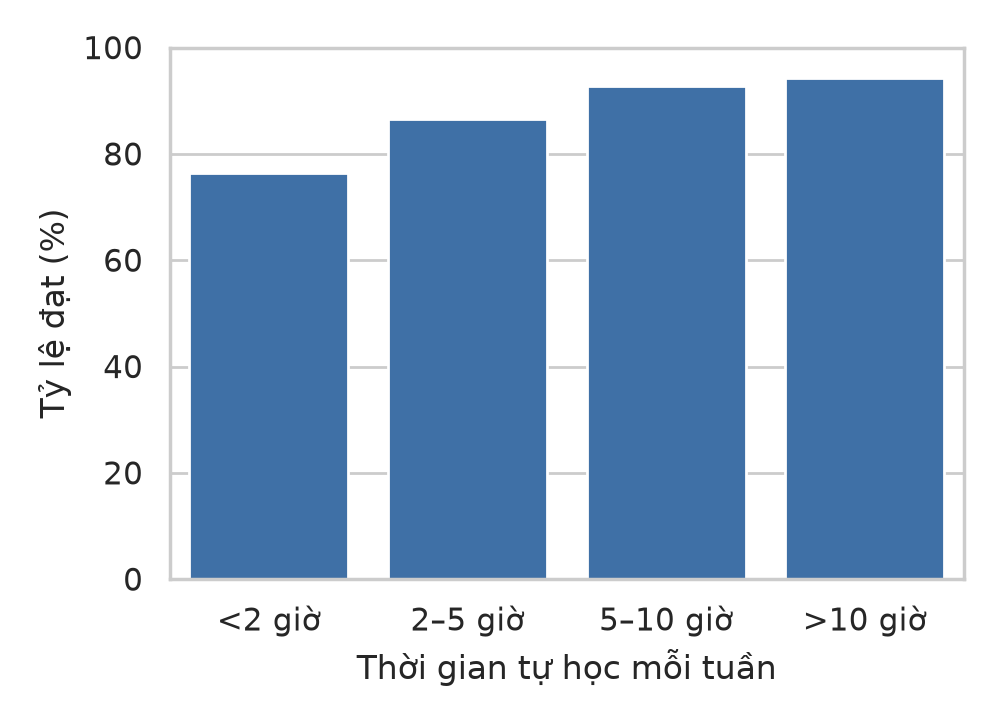
\includegraphics[width=0.48\linewidth]{eda_pass_by_studytime}}\\
\subfloat[Số buổi vắng và điểm $G_3$\label{fig:eda-abs}]{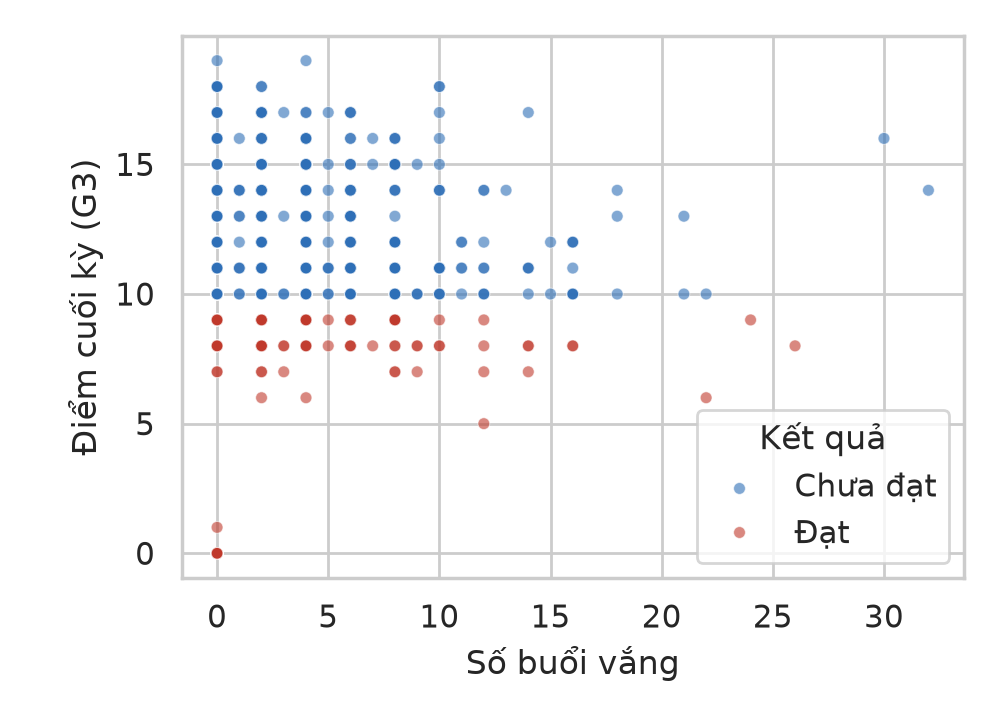
\includegraphics[width=0.48\linewidth]{eda_absences_g3}}\hfill
\subfloat[Ma trận tương quan\label{fig:eda-corr}]{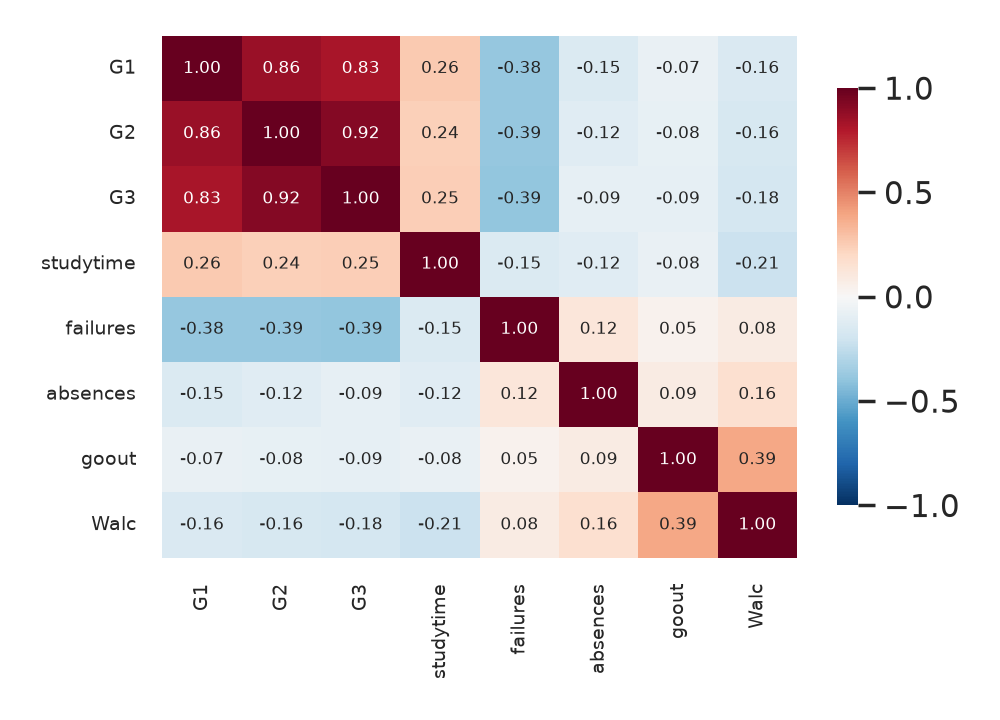
\includegraphics[width=0.48\linewidth]{eda_corr_heatmap}}
\caption{Khám phá dữ liệu: bốn hình con xếp hai hình mỗi dòng.}
\label{fig:eda}
\end{figure}

Hình~\ref{fig:eda-study} cho thấy tỷ lệ đạt tăng đều theo thời gian tự học, từ khoảng 76\%
lên 94\%. Hình~\ref{fig:eda-corr} cho thấy $G_3$ tương quan rất mạnh với $G_1$ và $G_2$, và
tương quan âm với số lần trượt trước đó.

% ------------------------------------------------------------
\section{Phương pháp}\label{sec:method}
\subsection{Cây quyết định}
Cây quyết định~\cite{quinlan1986} chia dữ liệu đệ quy theo thuộc tính làm giảm độ hỗn tạp
nhiều nhất. Với một nút chứa tỷ lệ $p_k$ mẫu thuộc lớp $k$, chỉ số Gini được tính theo
phương trình~\eqref{eq:gini}:
\begin{equation}\label{eq:gini}
  \mathrm{Gini} = 1 - \sum_{k=1}^{K} p_k^{2}.
\end{equation}
Chúng tôi dùng 16 thuộc tính đầu vào (không dùng $G_2$ để mô phỏng cảnh báo sớm), giới hạn
độ sâu 3, mỗi lá tối thiểu 10 mẫu, chia 70\% huấn luyện và 30\% kiểm tra có phân tầng.

\subsection{Gom nhóm K-Means}
K-Means~\cite{lloyd1982} tìm $k$ tâm cụm $\mu_j$ cực tiểu hóa tổng bình phương khoảng cách
trong cụm, theo phương trình~\eqref{eq:kmeans}:
\begin{equation}\label{eq:kmeans}
  J = \sum_{j=1}^{k} \sum_{x_i \in C_j} \lVert x_i - \mu_j \rVert^{2}.
\end{equation}
Sáu biến hành vi ($G_1$, thời gian tự học, số lần trượt, số buổi vắng, mức đi chơi, rượu bia
cuối tuần) được chuẩn hóa trước khi gom nhóm. Số cụm được chọn bằng phương pháp khuỷu tay và
hệ số silhouette~\cite{rousseeuw1987}.

\subsection{Hồi quy tuyến tính}
Điểm cuối kỳ được mô hình hóa là $\hat{G}_3 = \beta_0 + \sum_{j}\beta_j x_j$, đánh giá bằng
hệ số xác định $R^2$ và sai số tuyệt đối trung bình (MAE).

% ------------------------------------------------------------
\section{Kết quả và thảo luận}\label{sec:result}
\subsection{Phân loại Đạt/Chưa đạt}
Cây quyết định trong Hình~\ref{fig:tree} đạt độ chính xác 88,2\% trên 195 mẫu kiểm tra, F1
của lớp Chưa đạt là 0,66. Nút gốc tách theo $G_1 \le 8{,}5$: nhánh này chứa 13\% học sinh và
81\% trong số đó không đạt. Điểm $G_1$ chiếm 91\% mức độ quan trọng; số buổi vắng, số lần
trượt và mức đi chơi đóng vai trò phụ. Như vậy học sinh có $G_1$ thấp \emph{và} vắng nhiều hơn
8 buổi gần như chắc chắn không đạt.

\begin{figure}[t]
\centering
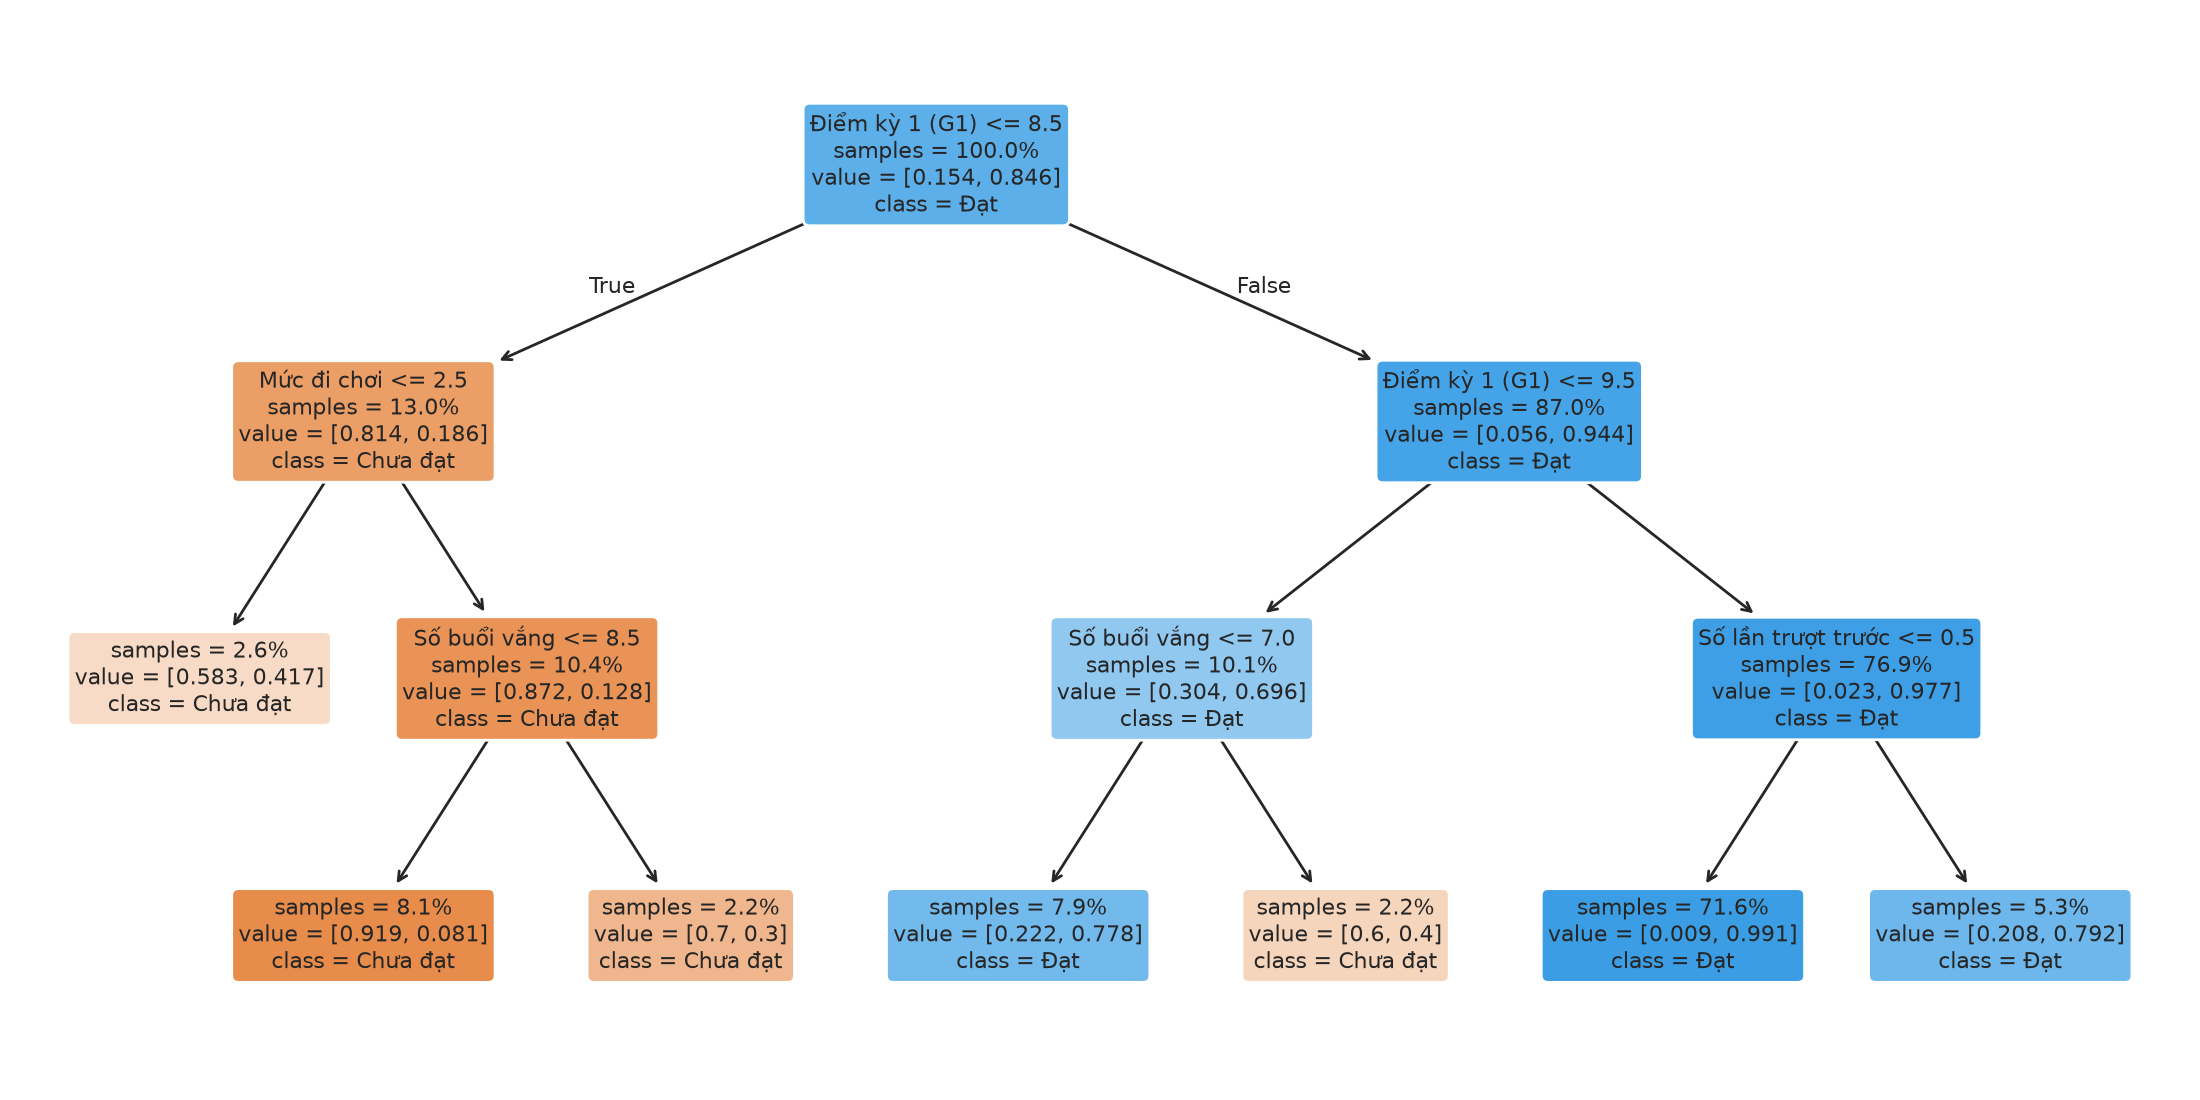
\includegraphics[width=\linewidth]{tree}
\caption{Cây quyết định độ sâu 3 phân loại học sinh Đạt/Chưa đạt.}
\label{fig:tree}
\end{figure}

\subsection{Phân nhóm người học}
Với $k=3$, ba cụm có đặc trưng rõ rệt (Bảng~\ref{tab:cluster}). Cụm 0 là nhóm rủi ro: điểm
$G_1$ thấp, trung bình trượt 1,5 lần và chỉ 45\% đạt. Cụm 1 có điểm trung bình nhưng đi chơi
và uống rượu bia nhiều. Cụm 2, chiếm hơn một nửa số học sinh, tự học nhiều, ít vắng và 95\% đạt.

\begin{table}[t]
\centering
\caption{Đặc trưng trung bình của ba cụm K-Means (cột rộng tự động theo nội dung).}
\label{tab:cluster}
\begin{tabularx}{\linewidth}{@{}l>{\raggedright\arraybackslash}X r r r r r@{}}
\toprule
Cụm & Mô tả & Số HS & $G_1$ & Trượt & Vắng & Đạt \\
\midrule
0 & Rủi ro: điểm thấp, từng trượt môn & 82  & 8,20  & 1,52 & 5,37 & 45\% \\
1 & Trung bình, đi chơi nhiều          & 206 & 10,64 & 0,06 & 5,49 & 82\% \\
2 & Chăm chỉ, ít vắng                  & 361 & 12,56 & 0,02 & 2,23 & 95\% \\
\bottomrule
\end{tabularx}
\end{table}

\subsection{Dự đoán điểm cuối kỳ}
Mô hình hồi quy dùng $G_1$, $G_2$, thời gian tự học, số lần trượt và số buổi vắng đạt
$R^2 = 0{,}883$ và MAE $= 0{,}75$ điểm. Hệ số của $G_2$ (0,85) lớn hơn nhiều so với các biến
còn lại, phù hợp với tương quan trong Hình~\ref{fig:eda-corr}.

\subsection{Thảo luận}
Kết quả nhất quán với các tổng quan~\cite{shahiri2015,albreiki2021}: điểm đánh giá trước đó
là yếu tố dự báo mạnh nhất. Ưu điểm của cây quyết định là các quy tắc dễ hiểu, giáo viên có
thể áp dụng trực tiếp. Hạn chế: dữ liệu mất cân bằng (15\% Chưa đạt) làm F1 của lớp thiểu số
chưa cao, và dữ liệu đến từ Bồ Đào Nha nên cần kiểm chứng trong bối cảnh Việt Nam.

% ------------------------------------------------------------
\section{Kết luận}\label{sec:conclusion}
Bài báo cho thấy chỉ với điểm kỳ đầu và vài chỉ báo hành vi, có thể nhận diện học sinh có
nguy cơ với độ chính xác trên 88\%. Hướng phát triển gồm: thử Random Forest~\cite{breiman2001},
cân bằng lớp, và thu thập dữ liệu học sinh Việt Nam có sự đồng ý và ẩn danh hóa đầy đủ.

\bibliographystyle{splncs04}
\bibliography{references}

\end{document}
